\subsubsection{Estimating accumulation}\label{accum}
The accumulation rate, $\dot{a}$, is highly uncertain for the Byrd ice core, so we compare ice flow model solutions using several accumulation functions. These include constant accumulation, a theoretical function derived for an expected atmospheric temperature timeseries at the nearby WAIS Divide ice core\citet{morse2002}, constant accumulation rates every 5,000 years, and constant accumulation rates in four depth bins which correspond to observed changes in layer thickness at the byrd ice core \citep{}. \textbf{Adding an accumulation function based on Byrd ice core isotopes.}

The result is shown in Figure \ref{fig:accumfunc}. We see that \textbf{One of them does better than the others. This one will be used in the final model to give the real result of age-depth for all the reflectors.}


%\begin{figure}
%%\begin{center}
%\centering
%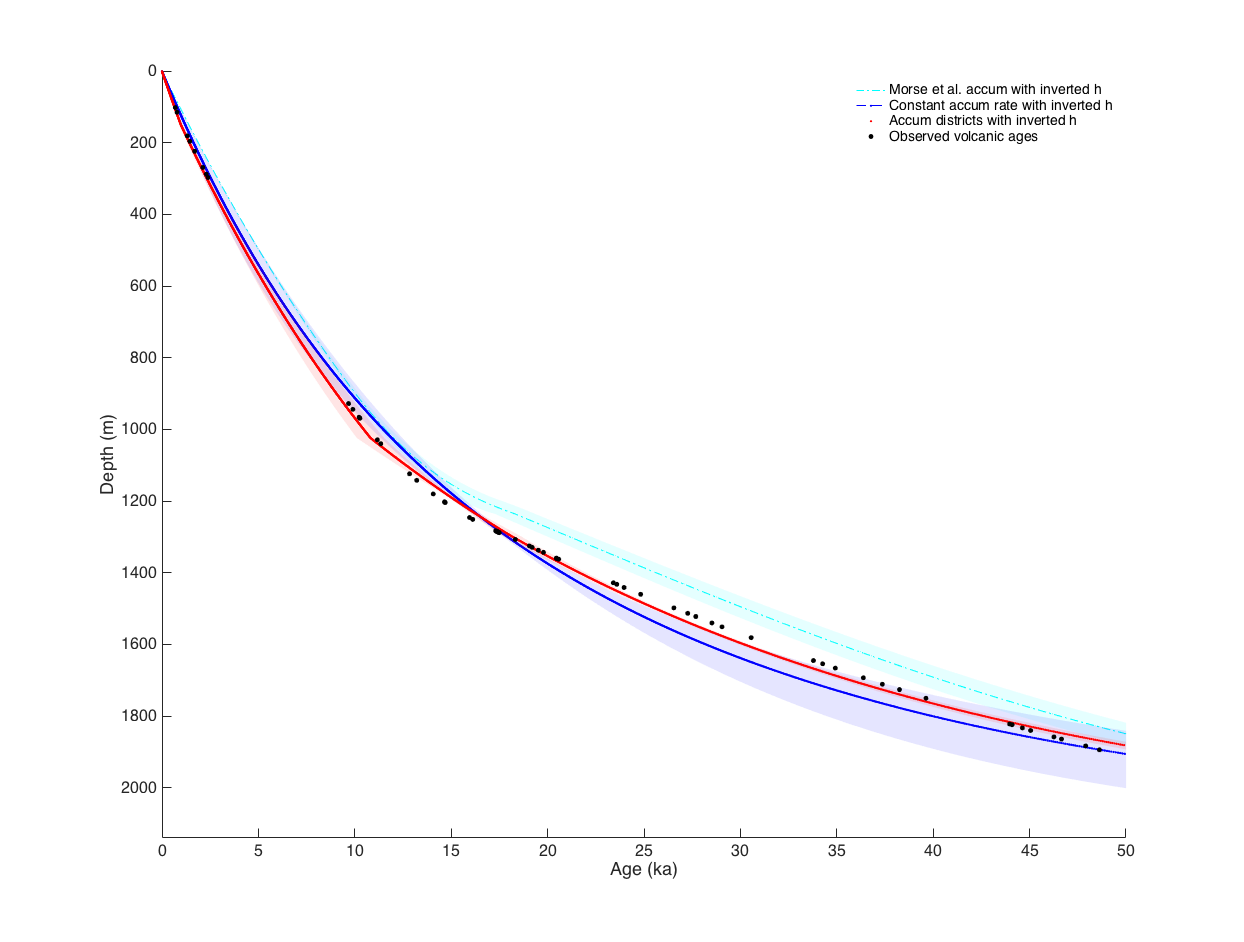
\includegraphics[scale=0.4]{figures/accumfunc}
%%\captionsetup{width=.9\textwidth}
%\caption[]{\textbf{Unfortunately, this figure is missing the 5k year interval which is the best (but takes the longest to run). In general, the accumulation functions fit the volcanic data well, but perhaps too well as seen in the comparison with the WAIS Divide ice core. This is a proof of concept that the data can be modeled using the MCMC method and we therefore can compute an age-depth profile even where there is no data, but the uncertainty so far is being underestimated.}}
%%\end{center}
%\label{fig:accumfunc}
%\end{figure}